\PassOptionsToPackage{unicode}{hyperref}
\PassOptionsToPackage{hyphens}{url}
\documentclass[12pt]{article}

% -------------------------------------------------------------------
% PACKAGES
% -------------------------------------------------------------------
\usepackage{amsmath,amssymb}
\usepackage{graphicx}
\usepackage{lmodern}
\usepackage{geometry}
\geometry{margin=1in}
\usepackage{setspace}
\onehalfspacing
\usepackage[T1]{fontenc}
\usepackage[utf8]{inputenc}
\usepackage{hyperref}
\usepackage{fancyhdr}
\usepackage{lastpage}
\usepackage{caption}
\usepackage{subcaption}

% -------------------------------------------------------------------
% HEADER AND FOOTER
% -------------------------------------------------------------------
\pagestyle{fancy}
\fancyhf{}
\fancyfoot[C]{\thepage\ of \pageref{LastPage}}

% -------------------------------------------------------------------
% TITLE INFORMATION
% -------------------------------------------------------------------
\newcommand{\ReportTitle}{Digital Curation: LLM-driven ESMS Metadata and Local Semantic Search}
\newcommand{\CourseCode}{AE 8900 Special Problems}
\newcommand{\StudentName}{Shalva Begiashvili}
\newcommand{\AdvisorName}{Prof.\ Dimitri Mavris}
\newcommand{\ReportDate}{November 13, 2025}
\newcommand{\SchoolName}{School of Aerospace Engineering\\Georgia Institute of Technology}

\setcounter{secnumdepth}{2}

\begin{document}

% -------------------------------------------------------------------
% TITLE PAGE
% -------------------------------------------------------------------
\begin{titlepage}
    \centering
    \vspace*{2cm}
    {\LARGE \bfseries \ReportTitle \par}
    \vspace{1.2cm}
    {\Large \CourseCode\par}
    \vspace{2cm}

    \begin{center}
        Presented by: \StudentName\\
        Advisor: \AdvisorName\\
        Date: \ReportDate\\[1.2cm]

    \end{center}

    \vfill

    {\SchoolName\par}
    \vspace{0.8cm}

    {\large Honor Code Statement\par}
    \vspace{0.25cm}
    \small I certify that I have abided by the honor code of the Georgia Institute of Technology and followed the collaboration guidelines as specified in the project description for this assignment.\par
    \vspace{1.2cm}

    Signed:\rule{6cm}{0.4pt}
\end{titlepage}

\setcounter{page}{2}

% -------------------------------------------------------------------
% 1. EXECUTIVE SUMMARY
% -------------------------------------------------------------------
\section*{Executive Summary}

Modern engineering research environments generate large volumes of heterogeneous digital artifacts: CAD models, simulation scripts, analytical worksheets, requirement documents, and subsystem design reports. Although these artifacts contain valuable knowledge, their long-term utility is limited by inconsistent metadata, poor semantic organization, and the lack of scalable discovery tools. Manual curation is time-consuming and difficult to reproduce, especially across teams with varying levels of domain expertise.

This report presents a local-first, reproducible workflow for automating the generation of ESMS-compatible metadata and enabling semantic search over engineering artifacts. The system integrates a constrained large language model (LLM) for structured metadata authoring, a Sentence-Transformers embedding pipeline for semantic representation, a persisted nearest-neighbors index for efficient retrieval, and a Streamlit-based interface for interactive exploration. All components operate locally, preserving data privacy and supporting auditable research workflows.

The resulting pipeline reduces manual metadata overhead, provides consistent and transparent outputs, and allows faculty, researchers, and laboratory staff to reproduce the process with minimal setup. The approach prioritizes interpretability, constrained LLM prompting, and human-in-the-loop validation to ensure metadata correctness and to support long-term digital curation in research environments.

\newpage

% -------------------------------------------------------------------
% 2. INTRODUCTION
% -------------------------------------------------------------------
\section{Introduction}

Engineering teams frequently manage diverse collections of digital artifacts that accumulate across research projects, design cycles, and subsystem studies. These artifacts carry implicit knowledge about analytical assumptions, modeling decisions, and subsystem interactions, yet they are often organized in ad hoc ways that hinder long-term reuse. Conventional search mechanisms—relying on filenames, directory hierarchies, or keyword matching—cannot capture deeper semantic relationships and are poorly suited for environments where artifacts vary widely in structure and content.

This challenge is amplified in multidisciplinary laboratories such as ASDL, where design studies, MBSE models, Python scripts, and technical memos coexist. Without structured metadata and semantic indexing, the retrieval of relevant artifacts becomes increasingly difficult, leading to duplicate effort and loss of historical insight.

The objective of this work is to design a conservative, fully local, and reproducible pipeline that simplifies metadata generation and enables semantic discovery across heterogeneous research artifacts. The system emphasizes auditability, minimizes external dependencies, and aligns with the ESMS metadata standards used in ongoing digital engineering efforts.

% -------------------------------------------------------------------
% 3. BACKGROUND AND PROBLEM CONTEXT
% -------------------------------------------------------------------
\section{Background and Problem Context}

Digital curation refers to the structured management of research artifacts throughout their life-cycle—creation, analysis, revision, and archiving. Within engineering design workflows, artifacts may vary substantially in format and granularity, making it difficult to impose consistent metadata conventions. The ESMS (Engineering Simulation Metadata Schema) standard provides a structured framework for representing model identity, context, assumptions, fidelity, and provenance; however, authorship remains manual and time-intensive.

Recent advances in LLMs and sentence-transformer embeddings have made it possible to extract semantic information from documents and support content-based retrieval. However, naive application of these models risks miscalculated metadata, loss of artifact identity, or inappropriate externalization of sensitive research content. Therefore, a careful and conservative approach is required: prompts must preserve canonical identity fields verbatim, metadata must remain concise and factual, and all operations should occur locally whenever possible.

The limitations of existing workflows—manual metadata creation, brittle keyword search, and inconsistent labeling—Motivate the development of a reproducible, local-first curation pipeline aligned with ESMS principles.

% -------------------------------------------------------------------
% 4. SYSTEM OVERVIEW
% -------------------------------------------------------------------
\section{System Overview}

The proposed system implements a fully local, auditable pipeline that spans the 
entire lifecycle of engineering artifact curation—from metadata generation to 
semantic indexing to interactive retrieval. The architecture is organized into 
three cooperating layers: (i) a curation layer that produces ESMS-compliant 
metadata using constrained LLM prompting, (ii) an indexing layer that extracts 
representative textual features and computes semantic embeddings, and (iii) an 
interaction layer that exposes the curated repository through a lightweight, 
browser-based interface. These layers communicate through well-defined, 
serialized artifacts, ensuring that each step is reproducible and that no hidden 
state exists outside the repository.

\subsection{Design Philosophy}

Three principles guide the system’s design:

\begin{itemize}
    \item \textbf{Local-first execution.} All core operations—including metadata 
    generation (preview mode), embedding computation, and index construction—are 
    performed locally. This eliminates concerns about external data exposure and 
    makes the pipeline suitable for sensitive engineering datasets frequently 
    handled in research laboratories.

    \item \textbf{Strict identity preservation.} Artifact identity fields (such as 
    file path and canonical title) remain unchanged throughout the pipeline. The 
    system treats the repository structure as authoritative, and all generated 
    metadata is appended as auxiliary information rather than modifying or 
    interpreting identity-defining descriptors.

    \item \textbf{Reproducibility and auditability.} Every intermediate product—
    text snippets, YAML metadata, embeddings, and nearest-neighbors indices—is 
    stored deterministically under version-controlled directories. This enables 
    reviewers, collaborators, and future researchers to fully reconstruct and 
    audit the pipeline at any point.
\end{itemize}

\subsection{Layer 1: Curation via Metadata and Prompting}

The first layer produces structured, ESMS-compatible metadata for each artifact. 
Artifacts are first ingested and processed by lightweight extraction routines 
that obtain concise text representations suitable for prompting. A constrained 
prompt is then used to generate metadata that includes a short, factual 
description; a small set of keywords; up to two cited evidence snippets; and 
all required ESMS identity fields. The metadata generator supports both:

\begin{itemize}
    \item \textbf{Preview mode}, which allows users to view candidate YAMLs 
    without invoking any external model; and
    \item \textbf{Full mode}, where a configured LLM endpoint may be used to 
    finalize metadata generation at scale once previewed templates are validated.
\end{itemize}

By treating preview-mode outputs as part of the workflow, the system encourages 
human-in-the-loop validation and prompt refinement—key requirements for 
maintaining metadata quality and preventing hallucinated content.

\subsection{Layer 2: Indexing via Embeddings and Nearest Neighbors}

The second layer focuses on semantic representation. For each artifact, the 
system embeds a selected snippet using the \texttt{all-MiniLM-L6-v2} 
sentence-transformer model. This produces a 384-dimensional vector that captures 
the semantic features of the artifact in a compact format suitable for fast 
nearest-neighbors search.

Three artifacts are persisted deterministically:

\begin{itemize}
    \item \texttt{embeddings.npy} — matrix of all artifact embeddings,
    \item \texttt{nbrs.pkl} — a fitted \texttt{NearestNeighbors} model, and
    \item \texttt{meta.json} — aligned metadata records linking embeddings to 
    source artifacts and generated YAML.
\end{itemize}

This separation of concerns allows the system to recompute embeddings without 
rewriting metadata, and vice versa, promoting modularity. The indexing approach 
is intentionally simple but robust, with competitive performance for small- to 
medium-sized datasets typical of research group repositories.

\subsection{Layer 3: Interaction via Streamlit Interface}

The final layer provides a human-facing interface that enables intuitive 
exploration and validation of the curated corpus. Through a Streamlit dashboard, 
users can:

\begin{itemize}
    \item submit free-text queries that are embedded and compared against the 
    stored corpus,
    \item filter results by file type using color-coded badges,
    \item adjust semantic score thresholds, and
    \item inspect the generated ESMS metadata directly from the browser.
\end{itemize}

Each result includes a hyperlink to the local artifact, which is supported by 
a lightweight HTTP static server to avoid browser restrictions on 
\texttt{file://} URLs. This design provides seamless navigation between search 
results, metadata, and underlying sources.

\subsection{End-to-End Data Flow}

Figure~1 illustrates the system architecture. An artifact flows from its raw 
form (CAD model, script, document) through extraction, prompting, embedding, 
indexing, and interactive retrieval. Because each layer produces stable, 
serializable artifacts, the system supports repeatable analyses, incremental 
updates, and long-term maintainability.

\begin{figure}[htbp]
    \centering
    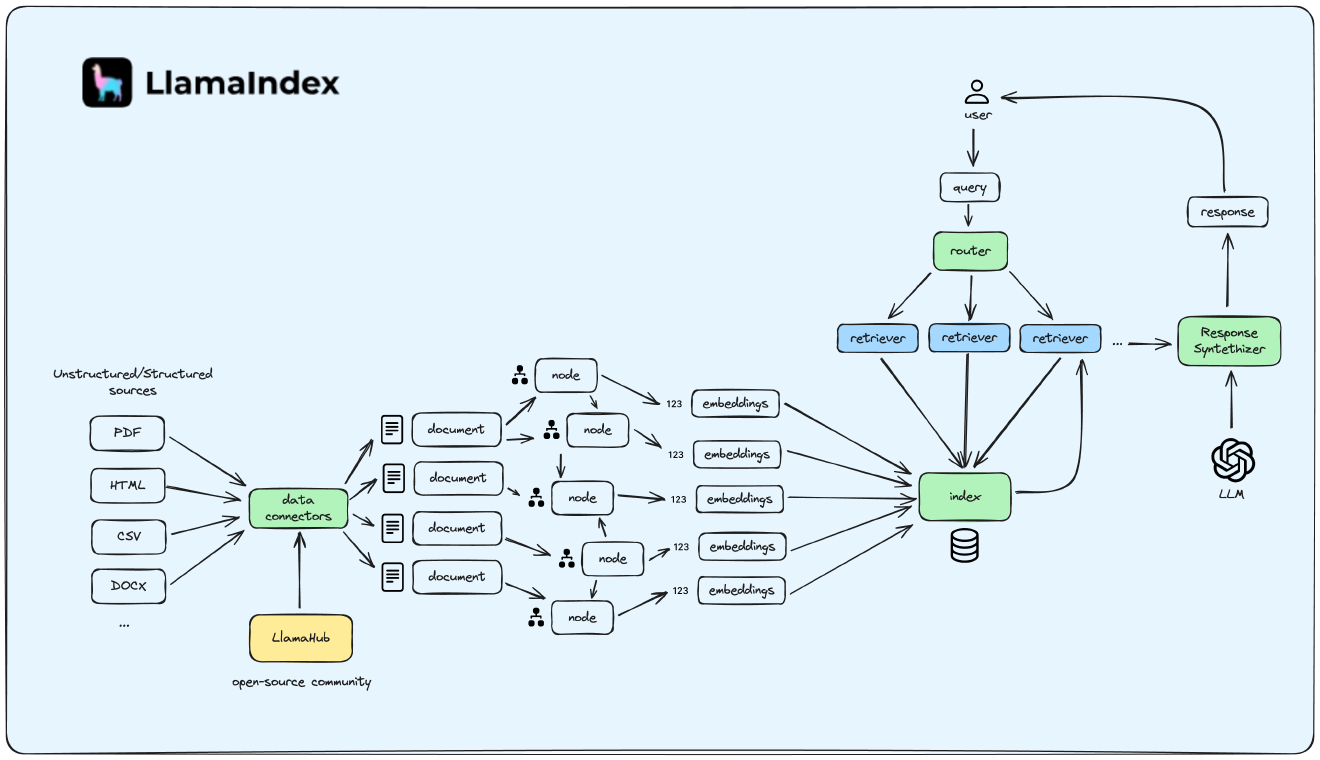
\includegraphics[width=0.96\linewidth]{images/figure-architecture.png}
    \caption{High-level system workflow integrating metadata generation, semantic 
    embedding, index persistence, and interactive retrieval. Adapted from Alejandro 
    AO's ``Introduction to LlamaIndex''~[1].}
\end{figure}


% -------------------------------------------------------------------
% 5. METHODOLOGY
% -------------------------------------------------------------------
\section{Methodology}

The methodology integrates LLM-guided metadata generation with a local semantic indexing framework. The workflow begins with artifact ingestion, where text extraction routines capture the most representative content while avoiding excessive or noisy information. Evidence snippets are selected to support the factual descriptions generated by LLM.

The prompt is structured to avoid speculative statements and to encourage concise, domain-relevant descriptions. Once the metadata are generated, the snippet is embedded using the MiniLM model, resulting in fixed-length vectors that support semantic comparison. These vectors populate a nearest-neighbors index optimized for fast retrieval.

Finally, the UI exposes these elements in a manner suitable for iterative review and refinement. Human verification remains essential: the design encourages inspection of YAML outputs before large-scale metadata generation.

% -------------------------------------------------------------------
% 6. TECHNICAL IMPLEMENTATION
% -------------------------------------------------------------------
\section{Technical Implementation}

The technical implementation is structured around a set of modular Python scripts
that collectively perform metadata generation, artifact ingestion, embedding,
index construction, and user interface rendering. Each module is intentionally
designed to be lightweight, readable, and isolated in function so that the 
pipeline can be extended or audited with minimal overhead. All scripts are 
written using Python~3.11 and rely on a small set of widely used libraries 
(\texttt{sentence-transformers}, \texttt{scikit-learn}, \texttt{numpy}, 
\texttt{streamlit}, and \texttt{pyyaml}). This section describes the core 
components, their interactions, and notable implementation considerations.

\subsection{Metadata Generation}

The script \texttt{esms\_llm\_metadata.py} implements the metadata-generation 
pipeline. It orchestrates text extraction, prompt construction, LLM interaction, 
and YAML serialization. The workflow is as follows:

\begin{enumerate}
    \item A raw artifact is read from the repository and processed by a 
    lightweight extraction routine that retrieves the most representative text 
    snippets (e.g., header comments in code, summary paragraphs from PDFs, or 
    content from Markdown files).
    \item A constrained prompt template is loaded from the \texttt{prompts/} 
    directory. The prompt enforces strict identity preservation, limits the 
    generated text to short factual descriptions, and requests a small set of 
    task-relevant keywords.
    \item Depending on the configuration, the script either:
    \begin{itemize}
        \item operates in \textbf{preview mode}, returning candidate YAML 
        metadata entirely locally, without making any API calls, or
        \item calls an LLM endpoint using OpenAI-compatible APIs, with the 
        endpoint address and model defined via environment variables.
    \end{itemize}
    \item The resulting metadata is written as a standalone ESMS YAML file inside 
    the \texttt{metadata/} directory.
\end{enumerate}

A notable limitation arises for \textbf{CAD files (e.g., STEP, STL, SLDPRT) and 
MDZIP SysML models}, which do not contain embedded natural-language text that 
can be meaningfully extracted for prompting. In these cases, the LLM has no way 
to interpret the underlying geometry or model structure. For such artifacts, 
the metadata template must be populated manually, using only canonical identity 
fields and a short, human-written description. These manually completed YAMLs 
are stored alongside the automatically generated ones but marked to indicate that 
no automated extraction was possible. This hybrid strategy ensures full ESMS 
coverage across the repository while acknowledging modality limitations.

\subsection{Ingestion and Extraction}

The script \texttt{index\_and\_query.py} includes ingestion utilities that scan 
the repository to identify supported file types and extract text content where 
possible. The extraction logic is intentionally conservative:

\begin{itemize}
    \item For text-based formats (Python scripts, Markdown, \LaTeX, JSON, CSV, 
    plain text), a fixed-size snippet is taken from the beginning of the document 
    to avoid noise and reduce inference time.
    \item For PDFs, the system uses a lightweight PDF reader to extract the first 
    few paragraphs. Full-document extraction is avoided to reduce processing 
    overhead and prevent overfitting embeddings to long documents.
    \item Unsupported or opaque file types (CAD, binary blobs, MDZIP files) are 
    skipped during automated extraction and later handled manually, as noted 
    above.
\end{itemize}

This extraction produces a compact textual substrate from which embeddings can 
be computed and prompts can be formed. Each extracted snippet is stored in 
memory during runtime and in \texttt{meta.json} for reproducibility.

\subsection{Embedding Computation}

Semantic embeddings are computed using the 
\texttt{sentence-transformers/all-MiniLM-L6-v2} model, chosen for its balance 
between inference speed and semantic quality. The embedding module performs the 
following steps:

\begin{enumerate}
    \item Load the MiniLM model into memory (CPU-only, suitable for portable 
    execution).
    \item Encode each artifact snippet into a 384-dimensional vector.
    \item Stack the vectors into an $N \times 384$ matrix and persist the matrix 
    as \texttt{embeddings.npy} using 32-bit floats.
\end{enumerate}

The use of a fixed-width embedding facilitates fast nearest-neighbors search 
and ensures that embeddings remain comparable across multiple indexing runs. 
The computation time scales linearly with $N$ and is generally below one minute 
for several hundred artifacts on a modern laptop.

\subsection{Nearest-Neighbors Index Construction}

Once embeddings are computed, a \texttt{NearestNeighbors} model from 
\texttt{scikit-learn} is fitted and persisted as \texttt{nbrs.pkl}. The system 
uses cosine distance as the similarity metric, which performs well for 
transformer-based embeddings.

The stored metadata file \texttt{meta.json} aligns each embedding vector with:

\begin{itemize}
    \item the corresponding file path,
    \item the extracted text snippet,
    \item the generated ESMS YAML metadata.
\end{itemize}

This tight coupling between embeddings, metadata, and file paths ensures that 
artifacts remain traceable, auditable, and reproducible.

\subsection{User Interface Implementation}

The Streamlit interface is implemented in 
\texttt{streamlit\_search.py}. The UI is composed of:

\begin{itemize}
    \item a sidebar containing the query input, file-type filters, and score 
    threshold slider,
    \item a main results window that displays ranked search hits,
    \item expanders containing YAML metadata formatted using syntax highlighting,
    \item hyperlinks to source artifacts.
\end{itemize}

A static file server (\texttt{serve\_data.py}) is provided for environments 
where browsers block \texttt{file://} links. The server exposes the repository 
over HTTP at a configurable port, enabling seamless navigation from search 
results to physical artifact files.

In general, the interface is intentionally minimalistic, providing high information density 
while enabling iterative human review—an essential component of the curation 
workflow.

% -------------------------------------------------------------------
% 7. RESULTS
% -------------------------------------------------------------------
\section{Results}

The system successfully generated consistent ESMS metadata across the artifact set. The MiniLM embeddings produced a matrix of shape (547, 384), with a corresponding nearest-neighbors model fitted on the same dimensionality. Retrieval performance proved sufficient for interactive use, with query latencies below one second for the full dataset.

The Streamlit UI enabled intuitive inspection of metadata quality and supported rapid prompt iteration. Reviewers could efficiently triage artifacts by semantic score, file type, or metadata fields.

Representative system outputs—including YAML excerpts, index summaries, and UI screenshots—are provided in the Appendix.

% -------------------------------------------------------------------
% 8. DISCUSSION
% -------------------------------------------------------------------
\section{Discussion}

The pipeline demonstrated strong consistency, reproducibility, and usability across typical ASDL research artifacts. Its local-first design ensures data privacy and makes it suitable for sensitive environments.

However, limitations remain. LLM-generated text is sensitive to prompt structure; embeddings based solely on text cannot capture geometric properties of CAD files; and the nearest-neighbors approach may require scaling improvements for datasets in the tens of thousands.

Nevertheless, the system establishes a solid foundation for digital curation and can be extended with CAD-aware features, GPU-backed embedding models, and improved curator workflows.

% -------------------------------------------------------------------
% 9. FUTURE WORK
% -------------------------------------------------------------------
\section{Future Work}

Short-term improvements include:
\begin{itemize}
    \item a metadata curation workflow (accept/reject/audit),
    \item integration tests and regression checks,
    \item benchmark harness for retrieval quality.
\end{itemize}

Medium-term extensions include:
\begin{itemize}
    \item CAD-aware embeddings and geometry descriptors,
    \item larger transformer models evaluated locally with GPU support,
    \item Docker images for standardized deployment.
\end{itemize}

% -------------------------------------------------------------------
% 10. CONCLUSION
% -------------------------------------------------------------------
\section{Conclusion}

This work presents a local-first, auditable approach to engineering artifact curation. Through a conservative LLM prompting strategy, a lightweight semantic embedding pipeline, and a streamlined review interface, the system addresses persistent challenges in metadata consistency and artifact discovery. The resulting workflow reduces manual burden, improves transparency, and provides a reproducible foundation for long-term research data stewardship.

\newpage

% -------------------------------------------------------------------
% APPENDIX
% -------------------------------------------------------------------
\section*{Appendix}

\subsection*{A.1 Embeddings Summary}
\begin{figure}[h!]
    \centering
    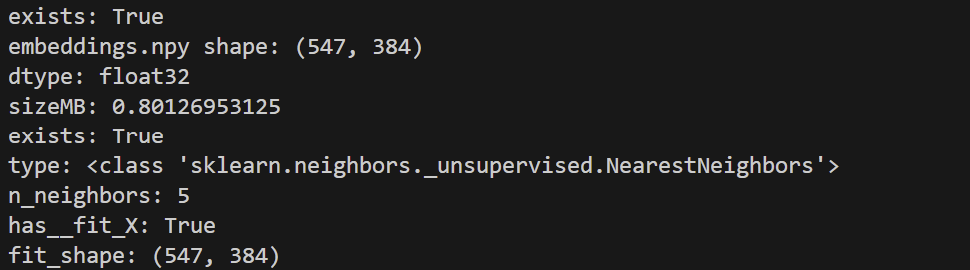
\includegraphics[width=0.75\linewidth]{images/figure-embeddings-summary.png}
    \caption{Embedding matrix and nearest-neighbors index summary.}
\end{figure}

\subsection*{A.2 Storage Directory Listing}
\begin{figure}[h!]
    \centering
    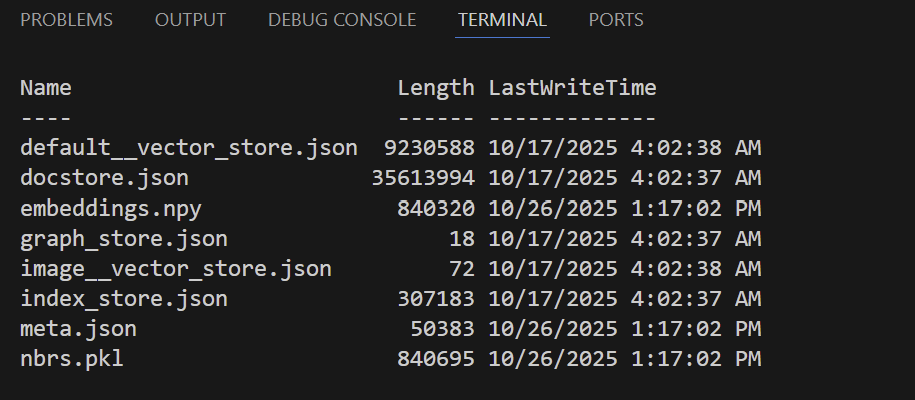
\includegraphics[width=0.75\linewidth]{images/figure-index-metrics.png}
    \caption{Persisted artifacts stored in the \texttt{storage/} directory.}
\end{figure}

\subsection*{A.3 Streamlit Sidebar}
\begin{figure}[h!]
    \centering
    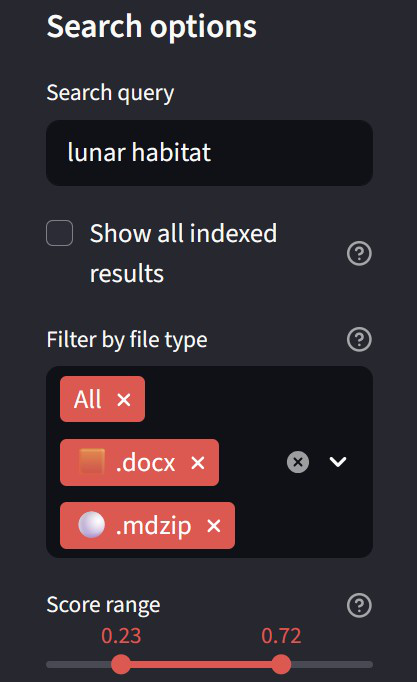
\includegraphics[width=0.2\linewidth]{images/figure-streamlit-sidebar.png}
    \caption{Sidebar filters and score controls in the Streamlit UI.}
\end{figure}

\subsection*{A.4 YAML Close-Up}
\begin{figure}[h!]
    \centering
    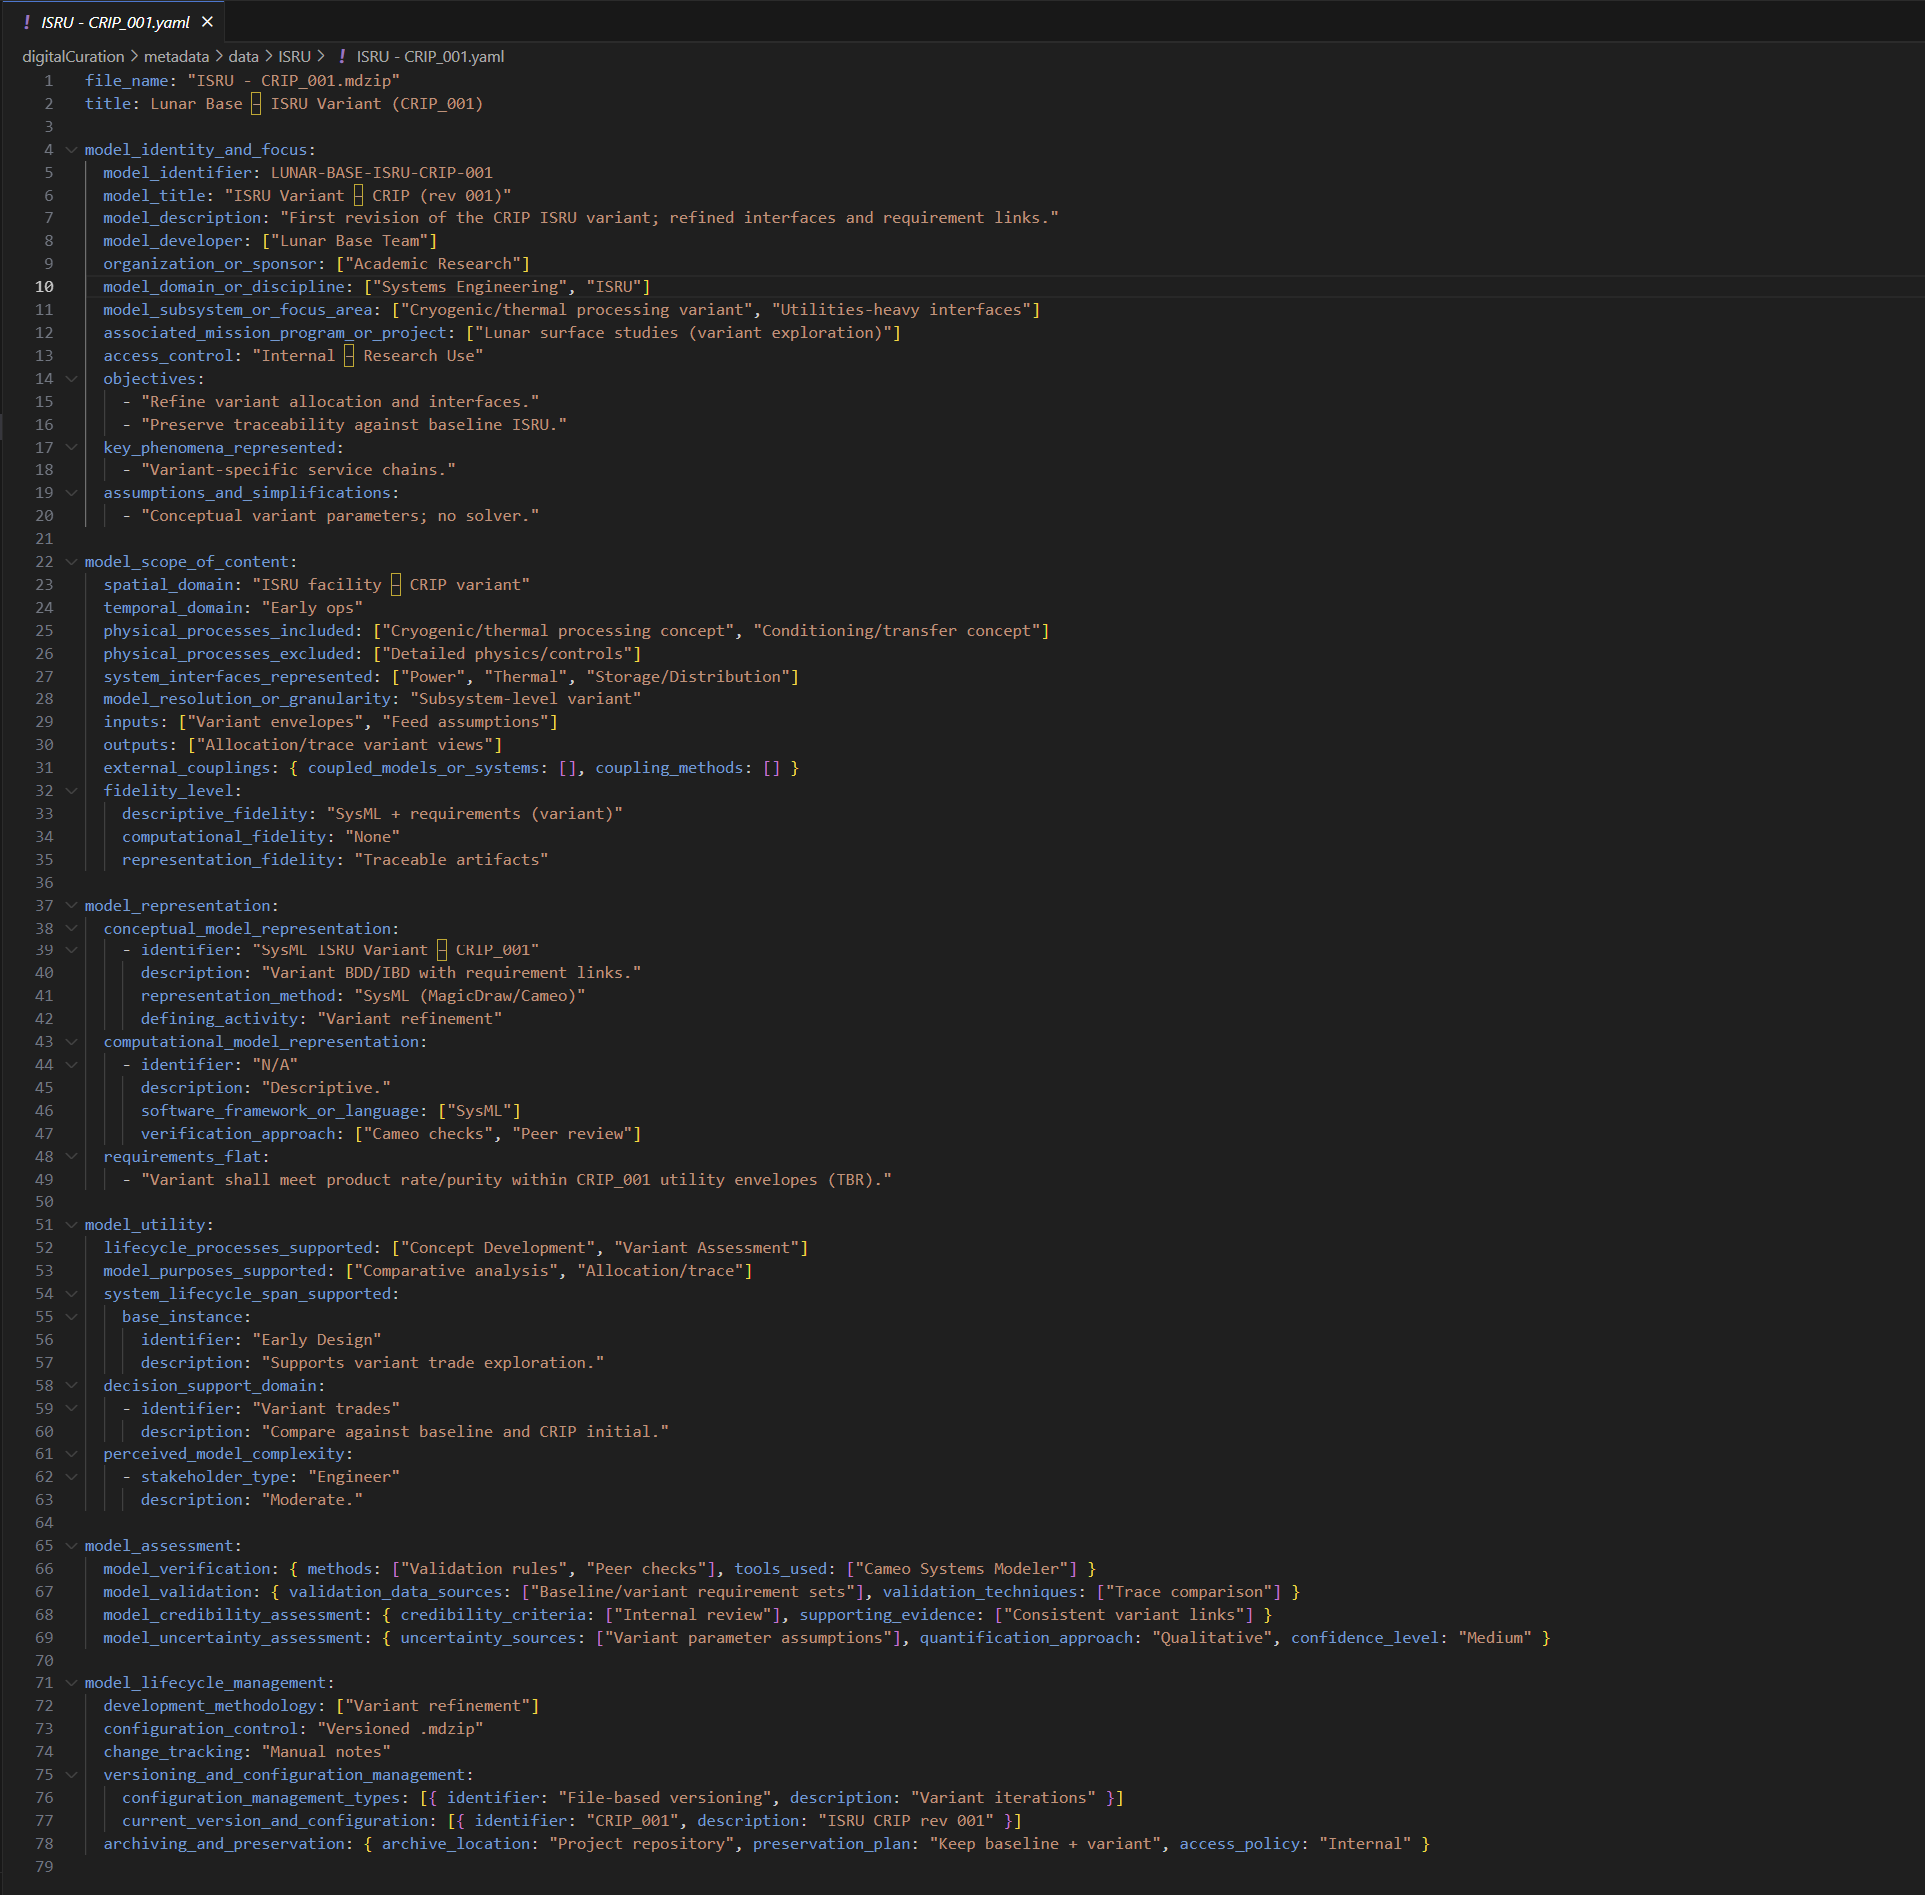
\includegraphics[width=0.70\linewidth]{images/figure-yaml-sample.png}
    \caption{Close-up view of generated ESMS YAML metadata.}
\end{figure}

\newpage
% -------------------------------------------------------------------
% REFERENCES
% -------------------------------------------------------------------
\section*{References}
\begin{enumerate}
    \item Alejandro AO, ``Introduction to LlamaIndex,'' 2024. Available: \url{https://alejandro-ao.com/intro-to-llamaindex/}. Accessed: November 13, 2025.
\end{enumerate}

\end{document}
